\documentclass[a4paper,12pt]{article}

% ===== Encoding & Language =====
\usepackage[T1]{fontenc}
\usepackage{lmodern}
\usepackage[utf8]{inputenc}
\usepackage[ngerman]{babel}
\usepackage[tracking=true,final]{microtype}
\usepackage{needspace}

% ===== Layout =====
\usepackage{geometry}
\geometry{margin=1in}
\raggedbottom
\usepackage{parskip}
\usepackage{graphicx}
\graphicspath{{./}{./images/}}
\usepackage[font=small,labelfont=bf]{caption}
\usepackage{float}

% ===== Header / Footer =====
\usepackage{fancyhdr}
\pagestyle{fancy}
\fancyhf{}
% Kopf- und Fußzeile anpassen
\fancyhead[L]{DevOps und Cloud Computing~3B – Milestone~1}
\fancyfoot[C]{Benjamin~Feichtlbauer et~al. – Seite \thepage}
\setlength{\headheight}{14pt}

% ===== Links & PDF meta =====
\usepackage[hidelinks]{hyperref}
\hypersetup{
  pdftitle={Infrastruktur-Spezifikation – Semesterprojekt DevOps und~Cloud~Computing~3B},
  pdfauthor={Benjamin~Feichtlbauer, Kevin~Forter, Mikulovic~Luka, Tepsurkaev~Abdulah},
  pdfsubject={Bachelor Informatik – DevOps und~Cloud Computing},
  pdfcreator={LaTeX}
}

% ===== Quick macros for repeating patterns =====
\newcommand{\pos}{\textbf{Positiv:} }
\newcommand{\negx}{\textbf{Negativ:} }
\newcommand{\impr}{\textbf{Verbesserungsvorschlag:} }

% Optional: compact itemize
\usepackage{enumitem}
\setlist{itemsep=2pt,topsep=4pt}

\begin{document}

% ===================== TITELBLATT =====================
\begin{titlepage}
  \centering
  \vspace*{2cm}
  {\Huge Infrastruktur-Spezifikation \par}
  \vspace{0.6cm}
  {\Large \textbf{Semesterprojekt – DevOps und~Cloud~Computing~3B} \par}
  \vspace{1.6cm}
  {\large Benjamin~Feichtlbauer (Teamleiter), Kevin~Forter, Mikulovic~Luka, Tepsurkaev~Abdulah\par}
  {\large Bachelor Informatik / 3.~Semester \par}
  {\large Lehrveranstaltung: DevOps und~Cloud~Computing~3B \par}
  {\large \today\par}
\end{titlepage}

% ===================== EINLEITUNG =====================
\section*{Einleitung}
In diesem Semesterprojekt planen wir die Infrastruktur für eine DevOps-basierte
CI/CD-Umgebung in der Amazon-Cloud. Die Infrastruktur soll ein privates
Netzwerk mit DNS-Auflösung, Versionsverwaltung, Continuous Integration,
Authentifizierung via LDAP sowie die Möglichkeit zur Ausführung von Pipelines
bereitstellen. Als Beispielanwendung wählen wir ein einfaches \LaTeX{}-Projekt:
ein hochgeladenes \texttt{.tex}-Dokument soll automatisch per GitLab-Pipeline
kompiliert und als PDF über eine \emph{saubere URL} bereitgestellt werden.
Dafür nutzt der GitLab-Runner NGINX zur Dateiauslieferung, und der GitLab-Server
veröffentlicht die PDFs per Reverse-Proxy unter \texttt{https://gitlab.\emph{<domain>}/pdf/…}.
Ziel dieser Spezifikation (Milestone~1) ist das Gesamtdesign: Topologie,
Dienste, Security-Regeln, Tests und Rollen.

% ===================== HAUPTTEIL =====================
\section*{Infrastrukturplanung}

Im Folgenden werden die für Milestone~1 geforderten Aspekte der
Infrastruktur spezifiziert. Für die grafische Darstellung der Topologie
verwenden wir Platzhalter; die konkreten Visualisierungen werden
im Laufe des Projekts erstellt.

\subsection*{Netzwerktopologie}

Die Projektumgebung besteht aus einer einzelnen Amazon VPC mit einem
\textbf{öffentlichen Subnetz} (IPv4-CIDR \texttt{10.0.0.0/24}). Alle Server
erhalten feste private IP-Adressen; nur der GitLab-Server besitzt eine
Elastic IP für den externen Zugriff. Interne Namensauflösung erfolgt über
die Zone \texttt{ci.intern}, die auf zwei DNS-Servern (primary / secondary)
repliziert wird. 

Die Architektur ist bewusst minimal gehalten:
GitLab dient als zentrales Gateway und Reverse-Proxy,
der Runner hostet NGINX zur Ablage der erzeugten PDFs,
und die DNS-Server stellen interne Erreichbarkeit sicher.
Ein optionaler LDAP-Server wird in Milestone 3 ergänzt.

\begin{figure}[H]
  \centering
  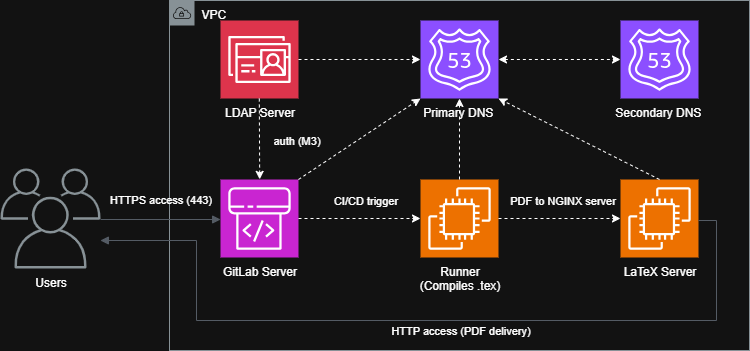
\includegraphics[width=0.95\textwidth]{assets/aws-diagramm-dark.png}
  \caption{Geplante Netzwerktopologie der CI/CD‑Umgebung}
\end{figure}


\paragraph{Interne Adressen und Namen:}
\begin{itemize}
  \item \textbf{primary.dns.ci.intern} – 10.0.0.10  | DNS (Zonenverwaltung)
  \item \textbf{secondary.dns.ci.intern} – 10.0.0.11  | DNS-Replikat / Failover
  \item \textbf{gitlab.ci.intern} – 10.0.0.20  | GitLab Server + Reverse-Proxy (TLS)
  \item \textbf{runner.ci.intern} – 10.0.0.21  | GitLab Runner + NGINX (PDF-Hosting)
\end{itemize}

\noindent
\textbf{Reverse-Proxy-Pfad:} GitLab veröffentlicht die unter
\texttt{/var/www/pdfs/\{dev,latest\}} auf dem Runner liegenden PDFs per
Reverse-Proxy als \texttt{https://gitlab.\emph{<domain>}/pdf/\dots}.

\subsection*{Sicherheitsgruppen}

Für jedes System wird eine eigene AWS-Security Group angelegt. Die
Inbound-Regeln sind strikt minimal; Outbound ist standardmäßig erlaubt.

\begin{itemize}
  \item \textbf{primary-dns-sg}: UDP/TCP~53 von \emph{runner-sg} und \emph{gitlab-sg};
        SSH (TCP~22) nur von Team-VPN/IP-Bereich.
  \item \textbf{secondary-dns-sg}: wie primary; zusätzlich Zonentransfer (IXFR/AXFR)
        von/zu 10.0.0.10.
  \item \textbf{gitlab-sg}: HTTPS (TCP~443) aus dem Internet, HTTP (TCP~80) nur Redirect;
        DNS (UDP/TCP~53) intern; SSH (TCP~22) nur Admins/VPN.
  \item \textbf{runner-sg}: HTTP (TCP~80) \emph{nur} aus \emph{gitlab-sg} (Reverse-Proxy);
        SSH (TCP~22) nur intern/VPN; DNS (53) intern. \emph{Keine} öffentliche Erreichbarkeit.
\end{itemize}

\subsection*{Services, Betriebssysteme und Pakete}

\begin{itemize}
  \item \textbf{DNS-Server (primary/secondary)}: Ubuntu~22.04~LTS, \texttt{bind9},
        \texttt{bind9utils}; Zone \texttt{ci.intern} (Forward/Reverse), Zonentransfer
        per IXFR/AXFR (kein manuelles rsync für Zonen!).
  \item \textbf{GitLab-Server}: Ubuntu~22.04~LTS, \emph{GitLab CE (Omnibus)}, Let’s-Encrypt-Zertifikat;
        optionale Elastic~IP (stabile öffentliche Erreichbarkeit).
  \item \textbf{GitLab Runner}: Ubuntu~22.04~LTS, \emph{gitlab-runner} (Docker-Executor),
        Docker Engine (20.10+); zusätzlich \emph{NGINX} zur Auslieferung der PDFs
        aus \texttt{/var/www/pdfs/}.
  \item \textbf{LDAP-Server (Milestone~3)}: OpenLDAP auf Ubuntu~22.04~LTS; Integration als
        Auth-Quelle für GitLab (Bind+Search); LDAPS optional/später.
\end{itemize}

\subsection*{Geplante Tests}

\paragraph{DNS}
\begin{itemize}
  \item Forward-Lookup: \texttt{dig gitlab.ci.intern @primary.dns.ci.intern} \(\to\) interne IP.
  \item Reverse-Lookup: \texttt{dig -x 10.0.0.20 @primary.dns.ci.intern} \(\to\) PTR korrekt.
  \item Forwarder: \texttt{dig google.com @primary.dns.ci.intern} \(\to\) Antwort vorhanden.
  \item Zonentransfer: \texttt{dig AXFR ci.intern @secondary.dns.ci.intern} \(\to\) Erfolg.
  \item Failover: primary stoppen \(\to\) \texttt{dig gitlab.ci.intern @secondary} liefert weiter Antworten.
\end{itemize}

\paragraph{GitLab Server}
\begin{itemize}
  \item Externer Zugriff: \texttt{https://gitlab.\emph{<domain>}} (TLS gültig).
  \item Repo anlegen, clone, push; Projekt sichtbar.
  \item Runner-Registrierung sichtbar (grüner Status im GitLab-UI).
\end{itemize}

\paragraph{Runner + NGINX (PDF-Bereitstellung)}
\begin{itemize}
  \item CI-Job kompiliert \LaTeX{} (\texttt{pdflatex} zweimal, non-stop-mode).
  \item Deploy-Job: Kopie der PDFs nach \texttt{/var/www/pdfs/\{dev,latest\}} via SSH/rsync.
  \item NGINX-Check (intern): \texttt{curl -I http://runner.ci.intern/pdf/latest/\emph{doc}.pdf} \(\to\) \texttt{200 OK}.
  \item Reverse-Proxy-Check (extern): \texttt{curl -I https://gitlab.\emph{<domain>}/pdf/latest/\emph{doc}.pdf} \(\to\) \texttt{200 OK}, \texttt{Content-Type: application/pdf}.
\end{itemize}

\paragraph{Security Groups}
\begin{itemize}
  \item Externes \texttt{nmap} auf GitLab-IP: nur 443 offen (80 Redirect).
  \item Interne Scans: runner nur von gitlab auf 80 erreichbar; dns nur intern.
\end{itemize}

\paragraph{LDAP (Milestone~3)}
\begin{itemize}
  \item \texttt{ldapsearch -x -H ldap://ldap.ci.intern -b "dc=ci,dc=intern"} liefert Test-User.
  \item GitLab-Login via LDAP-User möglich; Logs zeigen Bind/Search auf \texttt{ldap.ci.intern}.
\end{itemize}

\subsection*{Teamrollen und Verantwortlichkeiten}

\begin{itemize}
  \item \textbf{Benjamin~Feichtlbauer (Teamleiter)}: Projektkoordination, CI/CD-Pipeline,
        NGINX-Ablage + Reverse-Proxy-Konzept, Kosten-\& Risk-Abschätzung.
  \item \textbf{Kevin~Forter}: DNS (primary/secondary, Zone/Reverse, Transfer), Security-Groups,
        Unterstützung GitLab-Server (TLS/Omnibus).
  \item \textbf{Mikulovic~Luka}: Runner-Setup (Docker-Executor), NGINX-Konfiguration,
        SSH-Deploy-Pfad \texttt{/var/www/pdfs/\{dev,latest\}}, Hardening.
  \item \textbf{Tepsurkaev~Abdulah}: Schritt-für-Schritt-Dokumentation, Testfälle/Checklisten,
        Vorbereitung LDAP-Planung (Schema, User, Bind/Search).
\end{itemize}

\subsection*{Kostenabschätzung (vorläufig)}

Vier kleine Instanzen (\texttt{t3.micro}) + eine Elastic~IP (nur GitLab) + EBS (20–30\,GB/Instanz)
und geringer Traffic bleiben im Rahmen der 50\,USD AWS-Academy-Credits, wenn Instanzen
bei Nichtnutzung gestoppt werden. Detaillierte Kalkulation (AWS Pricing Calculator)
folgt in Milestone~3.

% ===================== FAZIT =====================
\section*{Fazit}
Die vorliegende Infrastruktur-Spezifikation legt das Fundament für den
Aufbau einer funktionsfähigen DevOps-Umgebung. Durch die kosteneffiziente
Topologie (eine VPC, ein Subnetz), klare Security-Groups sowie die
Konzentrierung der PDF-Auslieferung auf den Runner mit Veröffentlichung
über den GitLab-Reverse-Proxy erreichen wir ein professionelles, aber
budgetschonendes Setup. In den nächsten Meilensteinen setzen wir die
Planung auf AWS um, verifizieren DNS/GitLab/Runner, etablieren die
CI/CD-Stages und ergänzen LDAP; anschließend dokumentieren wir die
Schritte und demonstrieren die Funktion in Video und Präsentation.

\end{document}
